\documentclass{natureprintstyle}
%\documentclass{nature}
\bibliographystyle{naturemag}
\usepackage{epsfig,caption}
\usepackage{color}
\usepackage{bm}
\usepackage{graphicx}
\usepackage{longtable}
\usepackage{amssymb}
\usepackage{rotating}
\usepackage{latexsym}
\usepackage{hyperref}
\usepackage{float}

%\usepackage[switch]{lineno}
%\linenumbers

%%%%%%%%%%%%%%%%%%%%%%%%%%%%%%%%%%%%%%%%%%%%%%%%%%%%%%%%%%%%%%%%%%%
% comment for selecting the best figures to go on web for:
%@arxiver{jvds_sami_vsigma_ellip_LOESS_Age_paper.pdf,jvds_sami_vsigma_ellip_LOESS_Age_transform_paper_resubmit.pdf} 
%%%%%%%%%%%%%%%%%%%%%%%%%%%%%%%%%%%%%%%%%%%%%%%%%%%%%%%%%%%%%%%%%%%

%journal commands
\newcommand{\apj}{Astrophys. J.}
\newcommand{\spie}{Proc. SPIE}
\newcommand{\pasp}{Publ. Astron. Soc. Pac.}
\newcommand{\apjs}{Astrophys. J. Supp.}
\newcommand{\araa}{Annu. Rev. Astron. Astrophys.}
\newcommand{\mnras}{Mon. Not. R. Astron. Soc.}
\newcommand{\apjl}{Astrophys. J. Let.}
\newcommand{\aap}{Astron. Astrophys.}
\newcommand{\aj}{Astron. J.}
\newcommand{\nat}{Nature}
\newcommand{\na}{New Astron. Rev.}
\newcommand{\aaps}{A\&AS}
\newcommand{\procspie}{Proc. SPIE}

%%%%%%%%%%%%%%%%%%%%%%%%%%%%%%%%%%%%%%%%%%%%%%%%%%%%%%%%%%%%%%%%%%%
% my commands

\newcommand{\lcdm}{$\Lambda$CDM}
\newcommand{\hst}{{\it HST}}
\newcommand{\efr}{$R_{\mathrm{eff}}$}
\newcommand{\galfit}{{\sc Galfit}}
\newcommand{\mbh}{$\mathcal M_{\rm BH}$}
\newcommand{\lhost}{$L_{\rm host}$}
\newcommand{\jcap}{Journal of Cosmology and Astroparticle Physics}
\newcommand{\halpha}{${\it H}\alpha$}
\newcommand{\hbeta}{${\it H}\beta$}
\newcommand{\sersic}{S\'ersic}
\newcommand{\lenstronomy}{{\sc Lenstronomy}}
\newcommand{\reff}{{$R_{\mathrm{eff}}$}}
%\newcommand{\kms}{km~s$^{\rm -1}$}
\newcommand{\kms}{\ifmmode{\,\rm{km}\, \rm{s}^{-1}}\else{$\,$km$\,$s$^{-1}$}\fi}
\newcommand{\sigstar}{{$\sigma_*$}}
\newcommand{\mstar}{{$M_*$}}
\newcommand{\Mgii}{Mg$_{\rm II}$}
\newcommand{\Civ}{C$_{\rm IV}$}
\newcommand{\farcs}{\mbox{\ensuremath{.\!\!^{\prime\prime}}}}% fractional arcsecond symbol: 0.''0
%%%%%%%%%%%%%%%%%%%%%%%%%%%%%%%%%%%%%%%%%%%%%%%%%%%%%%%%%%%%%%%%%%%

\title{
%From predictions to observation: scaling relations between supermassive black holes and their host galaxies at $1< z<2$
A successful observational test of black hole and galaxy co-evolution models since $z\sim1.7$
%The first comparison between the observation and simulation of the scaling relations between supermassive black holes and their host galaxies at $1.2< z<1.7$
}
\author{Xuheng Ding$^{1,2}$, 
Tommaso Treu$^{1}$, 
John Silverman$^{2}$,
Tiziana Di Matteo$^{3}$,
et. al
}

\begin{document}

\maketitle

\let\thefootnote\relax\footnote{
\begin{affiliations}
\item {Department of Physics and Astronomy, University of California, Los Angeles, CA, 90095-1547, USA} 
\item {School of Physics and Technology, Wuhan University, Wuhan 430072, China}
\item {Kavli Institute for the Physics and Mathematics of the Universe, The University of Tokyo, Kashiwa, Japan 277-8583 (Kavli IPMU, WPI)}
\item{McWilliams Center for Cosmology, Dept. of Physics, Carnegie Mellon University, Pittsburgh PA 15213, USA}
\end{affiliations}
}

\begin{abstract}
Supermassive black holes (BH) harbor at the center of galaxies with their masses correlated to the properties of the host galaxies, known as scaling relations (\mbh-\lhost and \mbh-\mstar). Observational evidence indicates this correlation is evolving with cosmic time, suggesting a scenario that the BH growth predates their host. In theory, current simulations have reproduced the relations match very close to the observational sample at intermediate redshift ($0.3<z<1$) and local. Moreover, the positive evolution of the scaling relation is predicted by different simulating projects independently. It is important to make an unbiased comparison between the observations and the simulations at higher redshift ($z>1$), where the scaling relation is predicted to have a stronger evolution. To this end, here we use a large sample of 32 X-ray-selected broad-line (type-1) AGNs at $1.2 < z < 1.7$ ($\sim10$ billion years ago) and make the first comparison to the predicted sample from two state-of-the-art simulating projects, MassiveBlack-II (MBII) and semi-analytic models (SAMs). We use HST to measure the luminosity of the 32 AGNs in multi-bands, hence derive the trustworthy stellar mass measurements. The \mbh\ of our sample are estimated by the published near-infrared spectroscopic observations of the broad \halpha\ and \hbeta\ emission lines. We adopt the same selection function to obtain the comparison simulating sample, finding good agreements to the observational relations of \mbh-\lhost\ and \mbh-\mstar by the 32 AGNs. This consistency confirms the successful progress made by the simulations, which in turn would help to understand questions such as the origin of the scaling relation, the role of AGN feedback play, and the stellar components of galaxies which directly correlate to the BH growth.
\end{abstract}

\section{Introduction}
The discovery of the correlations between the masses (\mbh) of supermassive black holes (BHs) and the properties of their host galaxies, like stellar mass (\mstar) and luminosity (\lhost), indicates that the growth of BH is linked to its host galaxy formation. The best way to understand the physical mechanism of this connection is to rely on active galactic nuclei (AGN) and trace the scaling relations to higher redshifts, witnessing how and when does it happen. More recently, there is increasing observational evidence indicating the positive offset exist in the correlation at intermediate redshift range ($0.3<z<1$), implying that galaxies built up around the massive potential wells of mature BHs. Stimulated by the observations, theoretical efforts have been made to include the growth of \mbh\ in the framework of cosmological galaxy formation simulations, and generated the predictions of local scaling relations which match the observations well. Moreover, the simulations predict that the positive offset could be even stronger at redshift range $1<z<2$. 

Using the samples predicted by the simulation to compare to the observations is beneficial, in particular at high redshift. First, it helps to directly verify the validity of the initial physics prescriptions adopted in the simulation process, and point out the direction where to improve if needed. Second, in turn, the lessons learned in the simulations could be used to investigate the mechanism of the origin of the scaling relation. For example, the feedback originating in the surroundings of BHs, the major merging activities, and the growth of the \mbh\ and the stellar components as connected to the common gas supply have been invoked as the process leading to the co-evolution. Extending the comparison to high redshift help to explore the origin of the evolution directly. Furthermore, adopting the same selection function enable the particular comparison between two equivalent sample, so as to get rid of the systematic bias lead by the selection effects.

We study the scaling relations using 32 AGN systems selected from four X-ray coverage fields, including COSMOS \cite{Civano2016}, (E)-CDFS-S \cite{Lehmer2005, Xue2011}, and SXDS \cite{Ueda2008} fields at redshift range $1.2<z<1.7$. The redshift range of our targets is chosen to be high enough ($z>1$) to detect the existence of the evolution offsets, while low enough ($z<2$) to limit the effect of surface brightness dimming.
We employ the HST/WFC3 to obtain high-resolution imaging data and perform the 2-D flux profile decomposition to infer the light of the host galaxy. The X-ray selected sample have lower nuclear-to-host ratios at IR band, result in reliable host inference. 21/23 systems already have HST/ACS imaging data, which enable us to assess the host colors. We furthermore combining them with the ground-based photometry to carry out the SED fitting, and thus derive the reliable host rest-frame R band luminosity and stellar mass. The \mbh\ of our sample are estimated using the published near-infrared spectroscopic observations of the broad \halpha\ and \hbeta\ emission lines. These Balmer virial mass indicators remove the systematic with \Mgii\ or \Civ.

The high redshift measurements by our sample would place unique constraints on the cosmological simulations. To achieve this goal, we compare the observed scaling relations to the results from two state-of-art simulating projects, including MassiveBlack-II (MBII) and semi-analytic models (SAM). Note that the two projects are based on two independent simulating strategies, i.e. hydrodynamic simulation for MBII and semi-analytic model for SAM. The MassiveBlack-II (MBII) simulation is the highest resolution at the size of a comoving volume $V_{\rm box} = (100~{\rm Mpc}~h^{-1})$, including a self-consistent model for star formation, black hole accretion and associated feedback. The large simulation volume enables the simulating objects evolve independently; the high enough mass and spatial resolution meet the requirements for the object details. On the theoretical side, aimed, high-resolution N-body simulations can study specific galaxy systems. However, understand the mechanism of the scaling relation requires an analytical description of such processes to be implemented into existing semi-analytic models, such as (SAM). 
The successful predictions have been made by MBII and SAM in previous works \cite{Menci2014, Menci2016, Khandai2015}. We refer the interested readers to these works for more details.

\section{Results}
In figure~\ref{fig:MBII_comp}, we present the comparison between the observational measurements to the predictions from MBII, including the scaling relations of \mbh-\lhost and \mbh-\mstar. The samples from the simulation are chosen based on a same selection function in figure~\ref{fig:selectfunc}. Inspiringly, we find that the simulation matched remarkably well to the observing result. 

\begin{figure*}%[!b]
\begin{tabular}{c c}
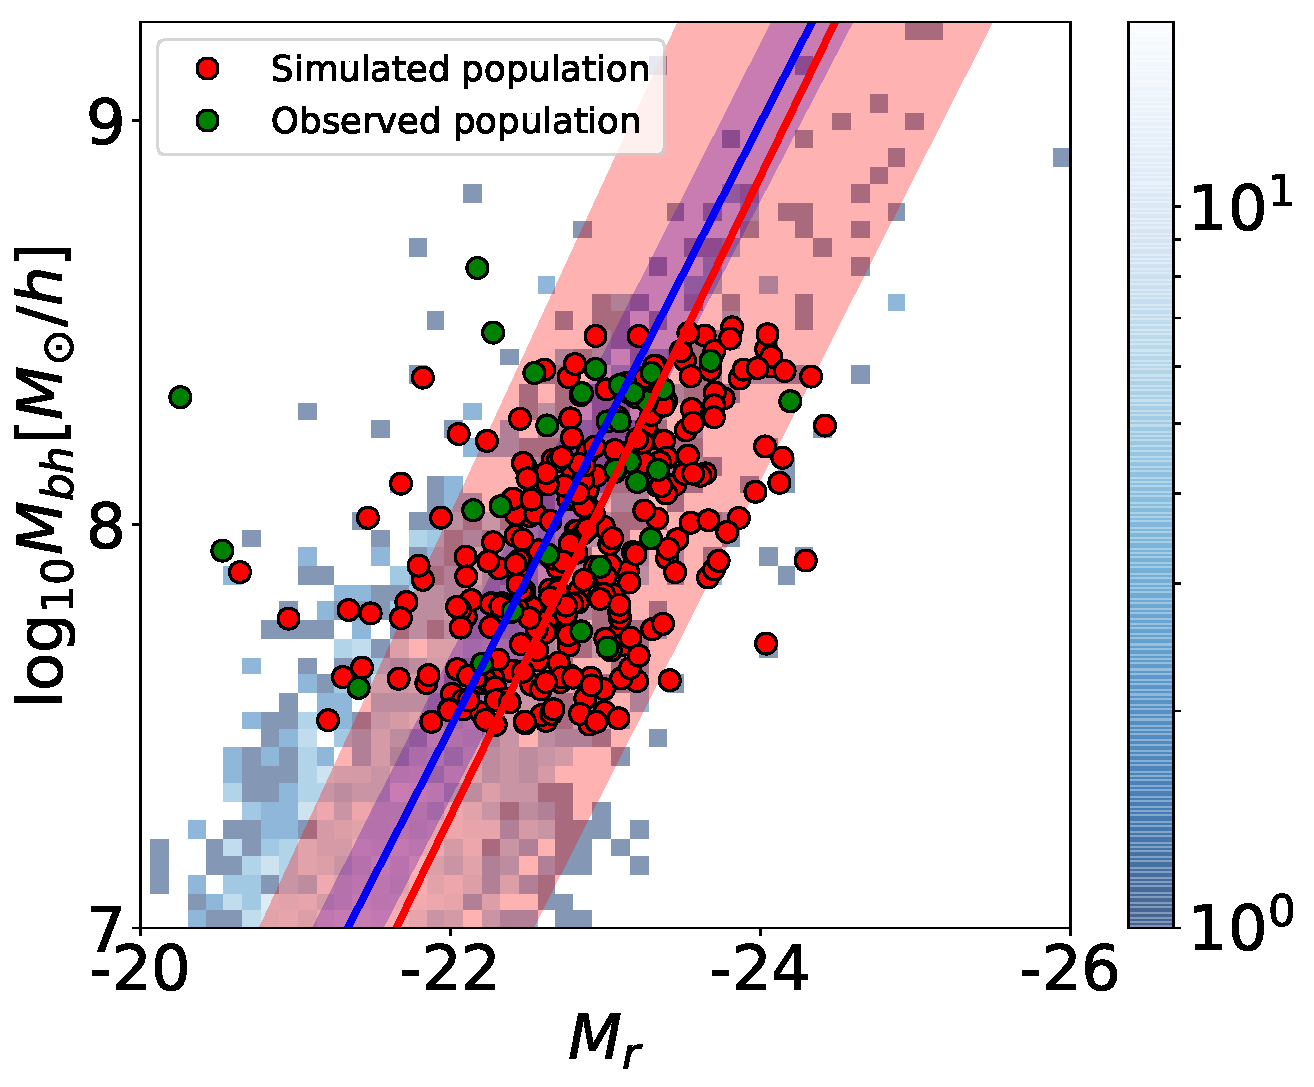
\includegraphics[width=0.5\linewidth]{MBII_ML.pdf} &
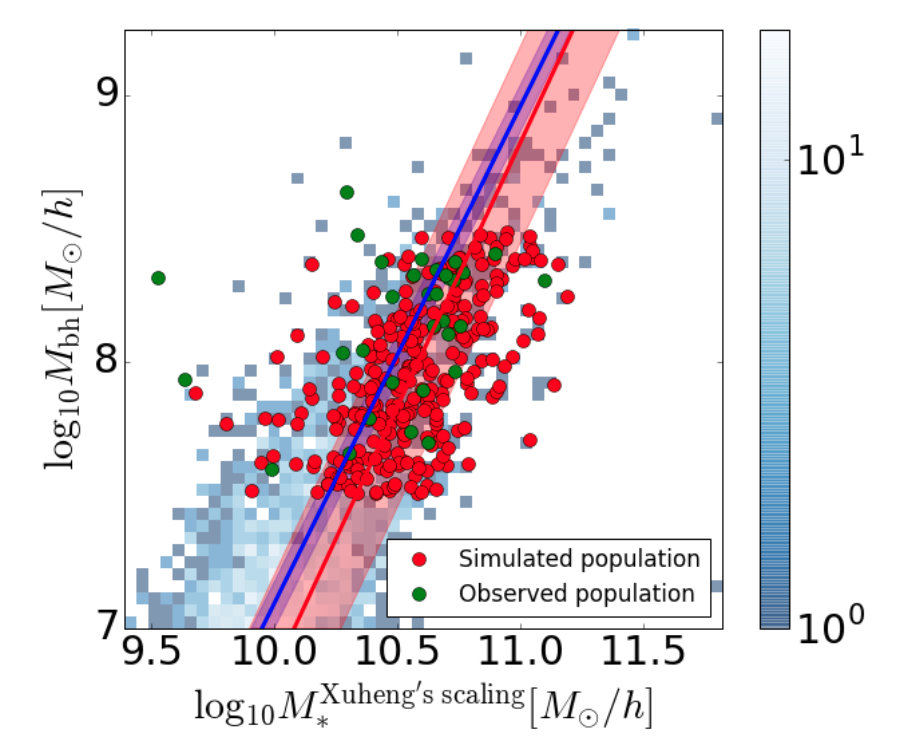
\includegraphics[width=0.5\linewidth]{MBII_MM.png} \\
\end{tabular}
\caption{
Comparing the scaling relations between the observed samples to the predicted samples by the MBII simulation. In the left and right panel, we present the \mbh-\lhost\ and \mbh-\mstar correlation, respectively. The blue grids are all galaxies that predicted in the MBII simulation. We find that the observations are perfectly overlapped with the simulations. 
}
\label{fig:MBII_comp}
\end{figure*}

\begin{figure*}[t]
\begin{tabular}{c c}
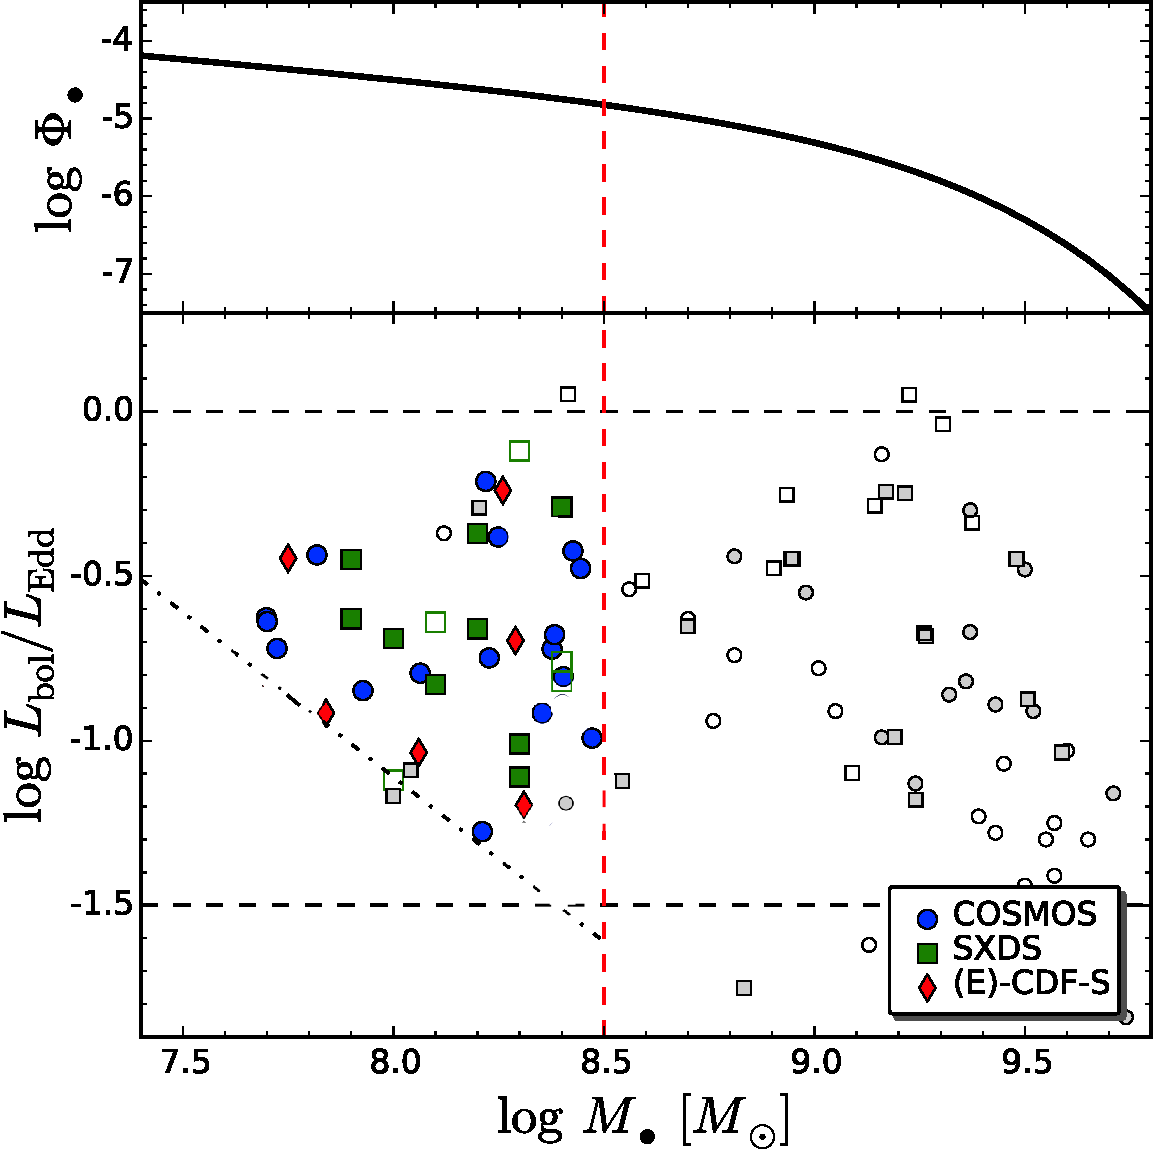
\includegraphics[width=0.5\linewidth]{hst_sample_bhmf.pdf}&
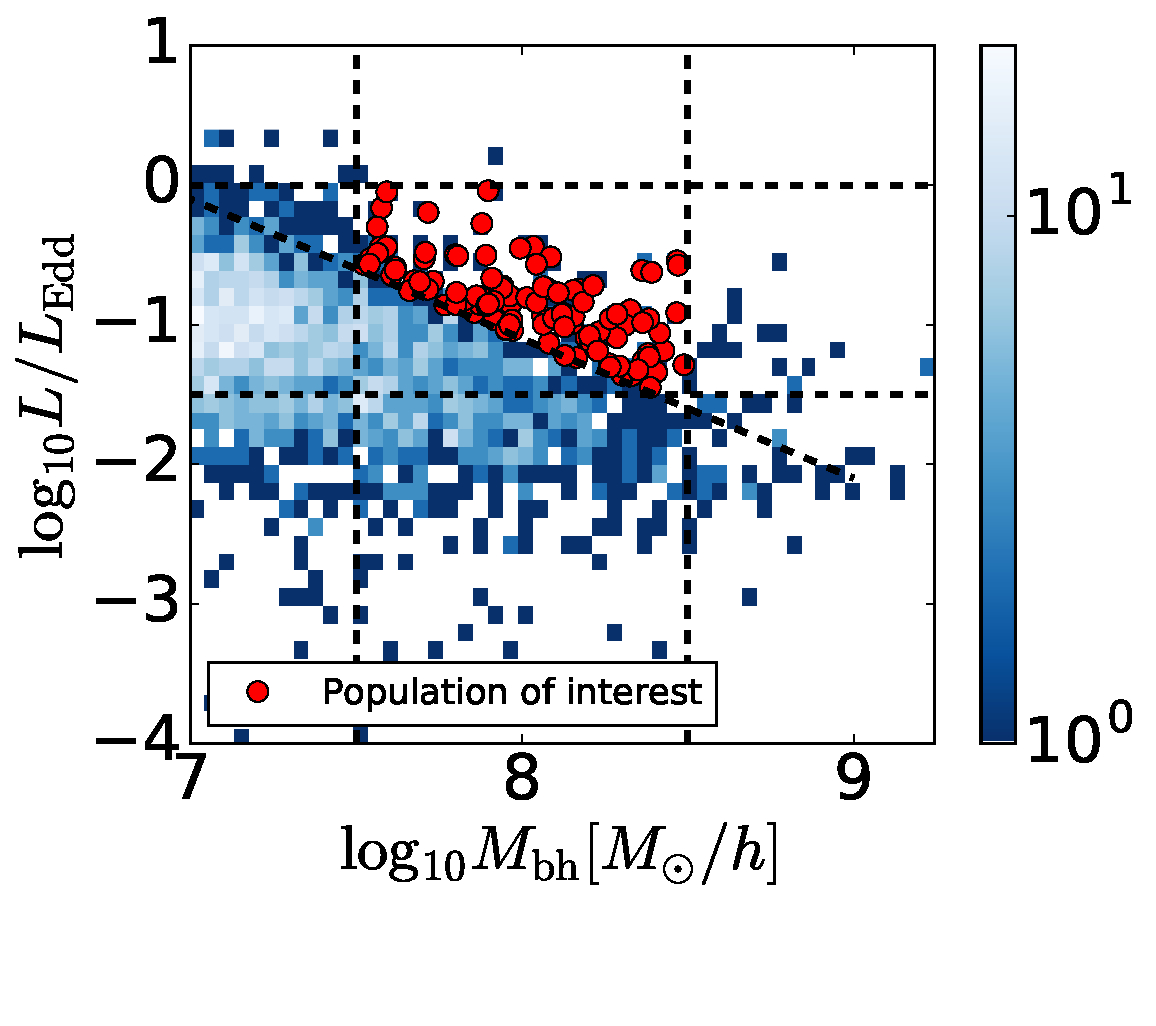
\includegraphics[width=0.5\linewidth]{MBII_selectfunc.pdf} \\
\end{tabular}
\caption{The selection function for the 32 AGN sample (left) and the predicted sample by MBII (right).
}
\label{fig:selectfunc}
\end{figure*}

In addition, we compare the observed measurements to the SAM simulation in figure~\ref{fig:SAM_comp}. The results also demonstrate a very consistency between the prediction by the model to the observation.

\begin{figure*}%[!b]
\begin{tabular}{c c}
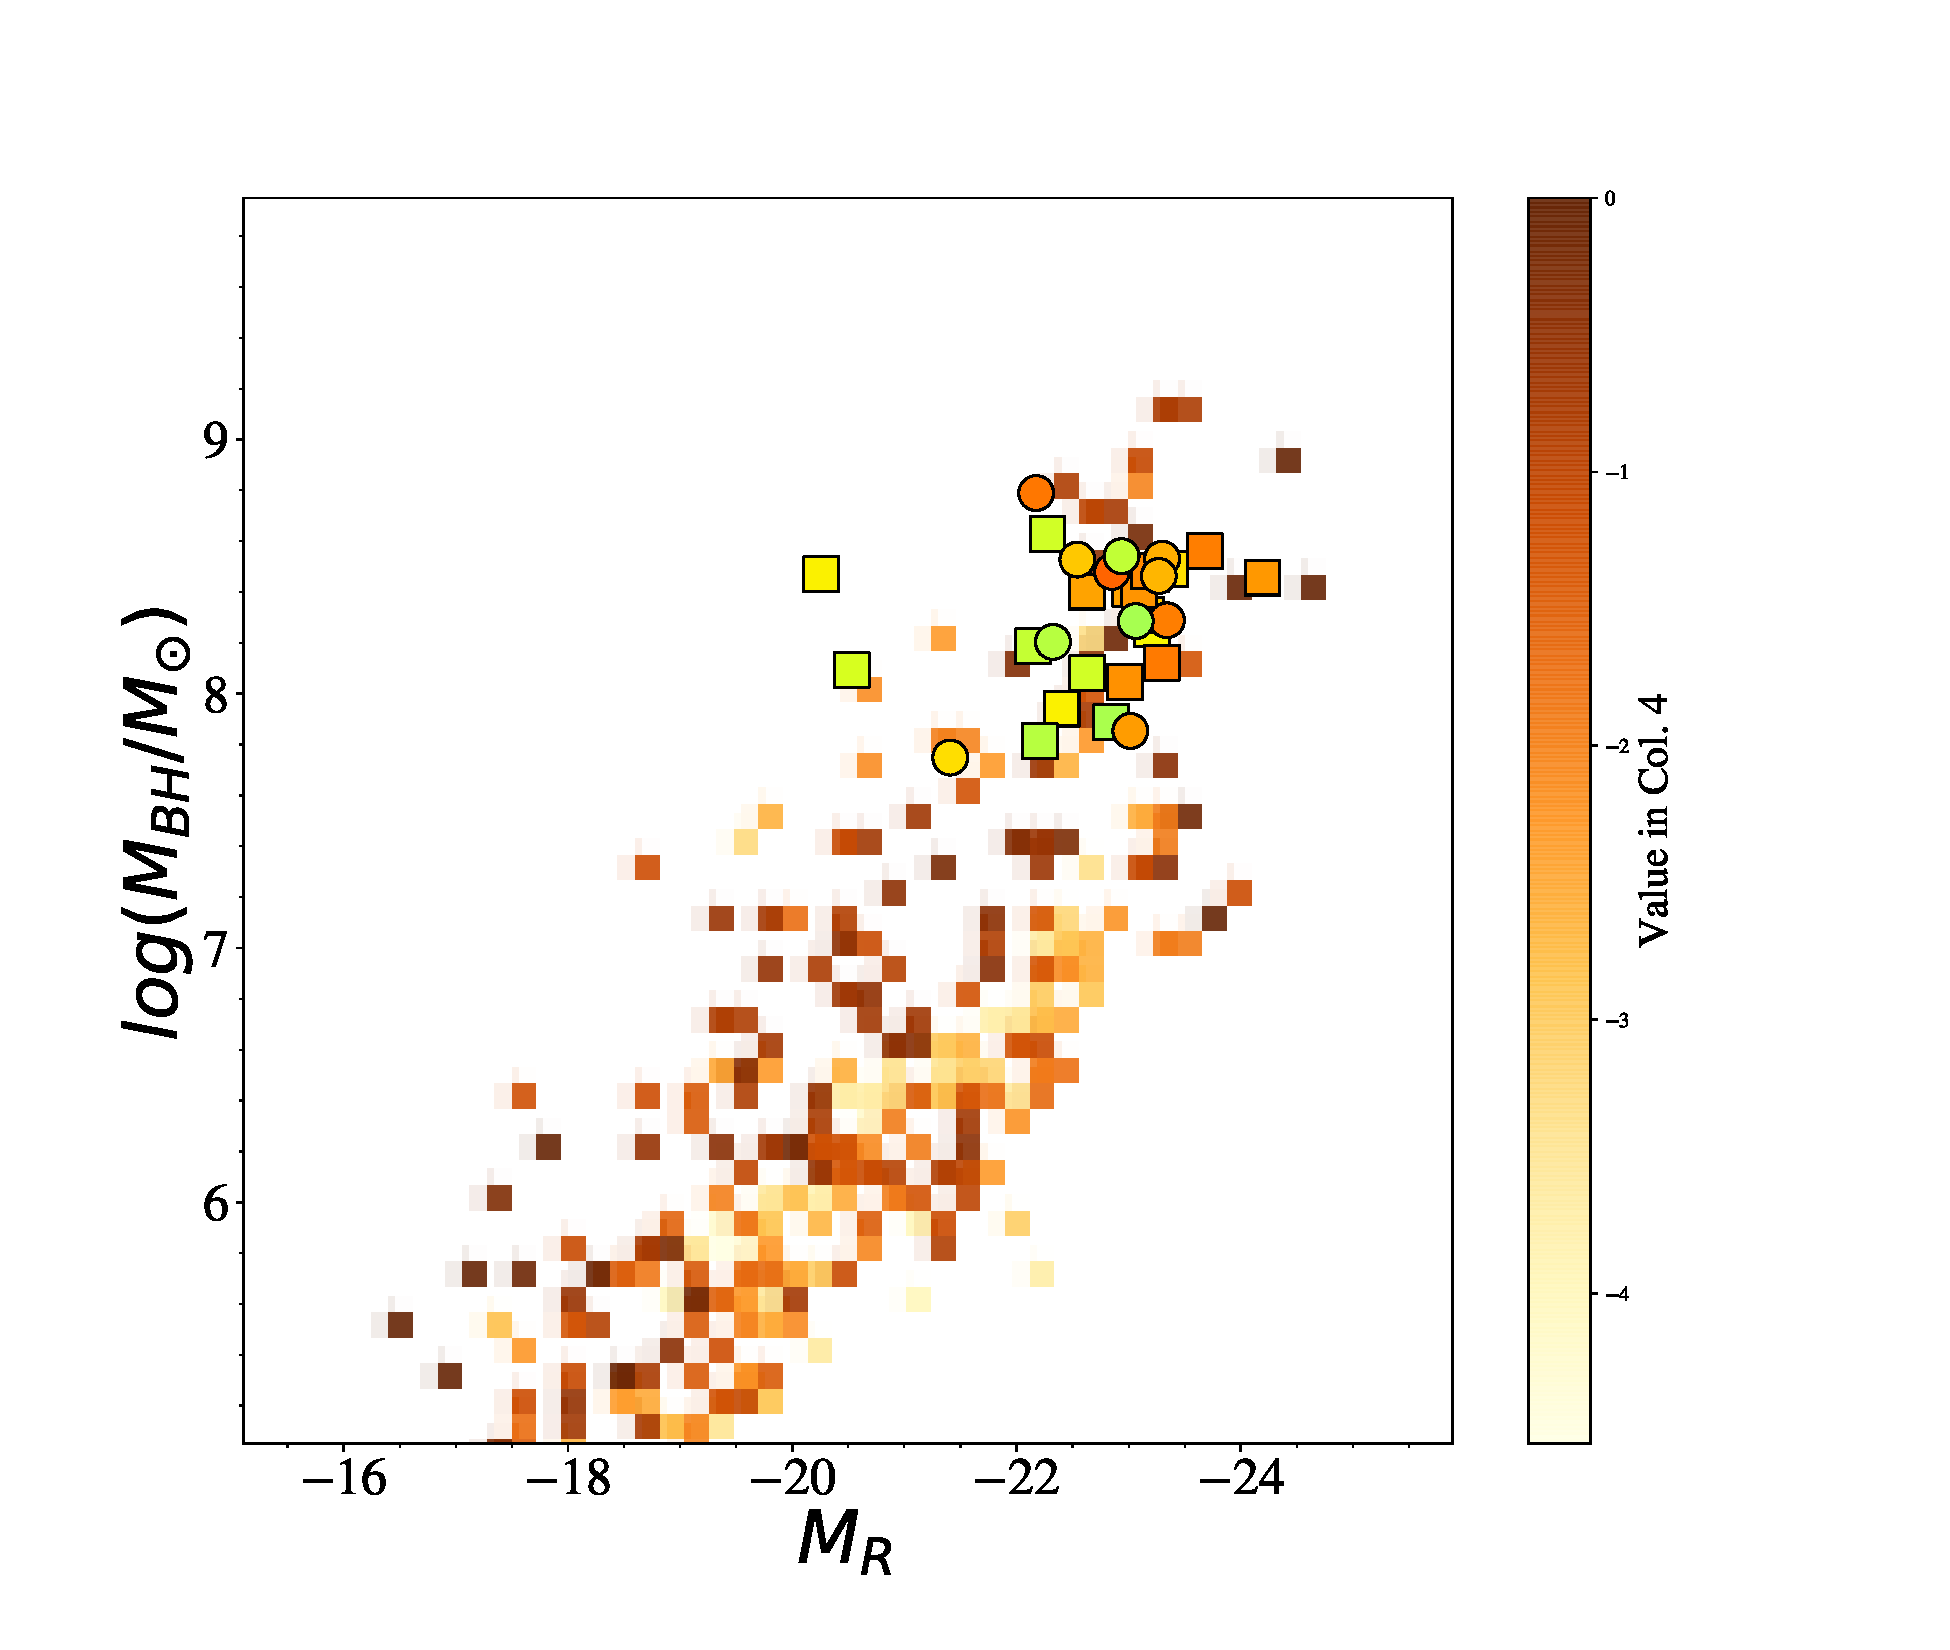
\includegraphics[width=0.5\linewidth]{SAM_ML.pdf} &
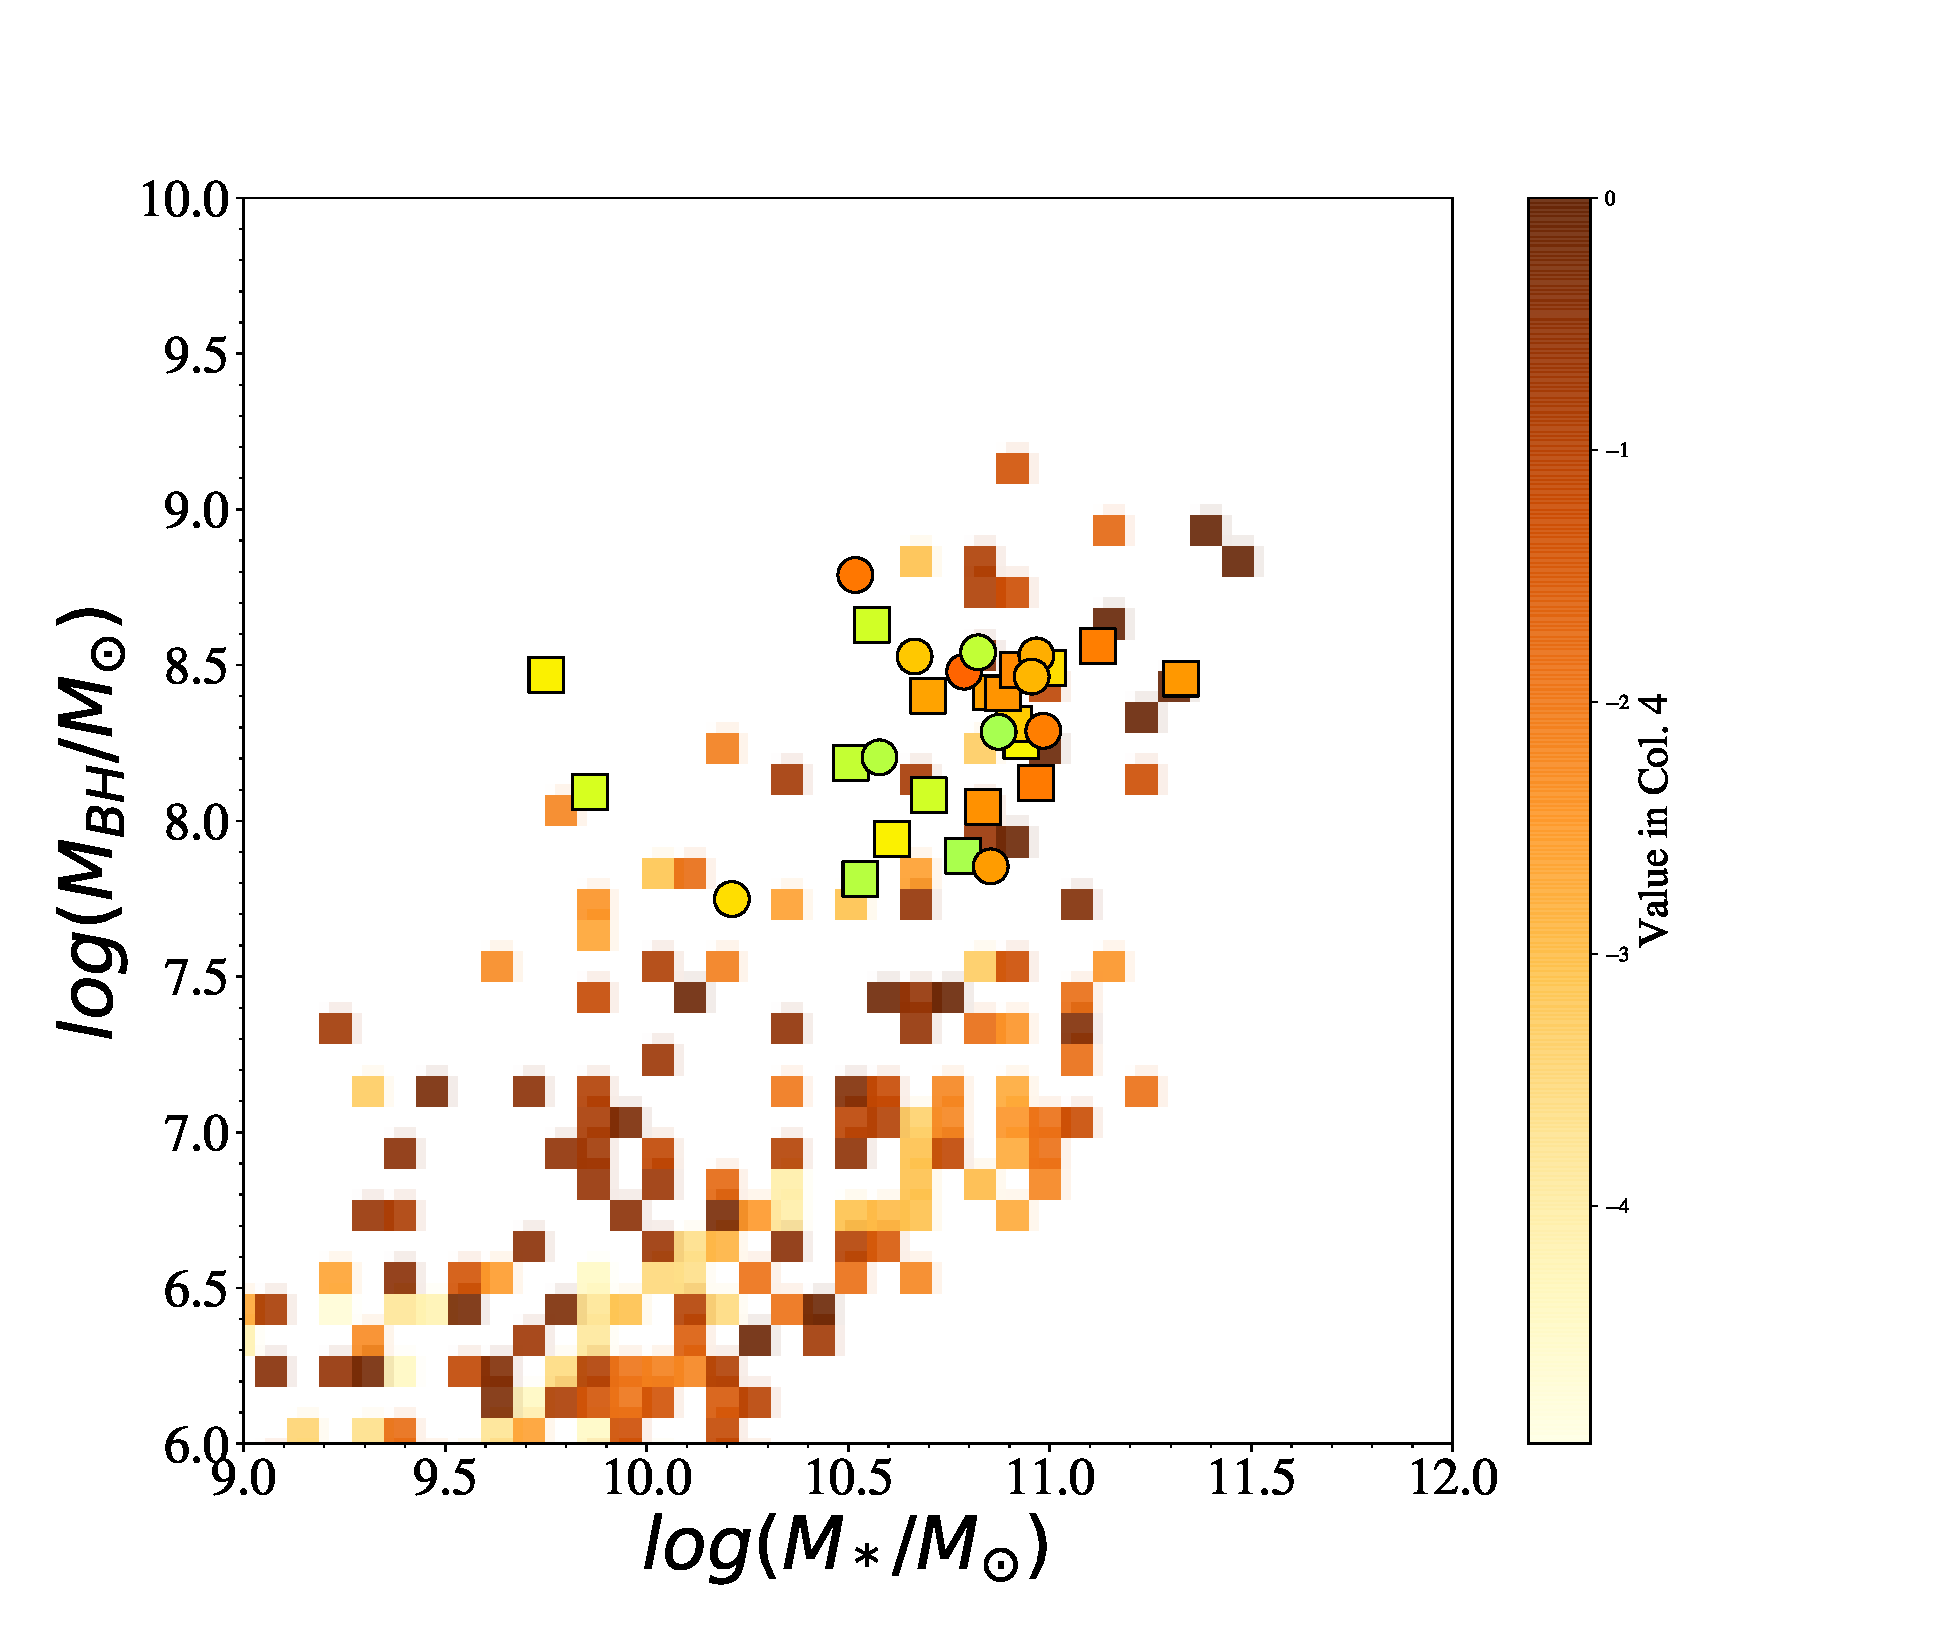
\includegraphics[width=0.5\linewidth]{SAM_MMstar.pdf} \\
\end{tabular}
\caption{
Comparing the observation to the SAM simulation.
}
\label{fig:SAM_comp}
\end{figure*}

\textcolor{blue}{The details of the results could be presented.\\
0. Compare the color of the sample?\\
1. 2D KS test? \\
2. More insightful inference from the comparing?
}

%Discuss the result, What does this mean?
The excellent match between the prediction of simulation and the observations highlights that the evolving scenario of the scaling relation is likely exist. In the distant Universe, the BHs at higher redshift typically reside in lower stellar mass galaxies than today. During this co-evolution process, in order to catch up on the local final relation, the stellar mass of the host galaxy would have to grow faster than its center BH.

 \textcolor{blue}{If the final results show such feature:}
The result also shows that the \mbh-\mstar\ relation has less scatter than the \mbh-\lhost\ relation, suggesting that the BH relation with \mstar\ are more fundamental than \lhost.

This successful experience leads one conjecture that the other prediction by the simulations could likely to be right. For example, regarding the stellar components of galaxy which is the origin that related to the growth of BH, it is likely that the bulge masses are tightly related.

\section{Discussion}
Some discussions should be placed in this section.

On the observation side:\\
0. The inferred host flux ratio by SED decomposition is consistent to the 2-D image decomposition, indicating the fidelity of these approaches?\\
1. HST seems to reach its higher limit. In the future, the JWST is very promising to realize the evolution scenario at even higher redshift.\\


On the simulation side:
\\0. Introduce some the other 
\\1. How do we discuss the role of AGN feedback?.

\clearpage
\newpage

\begin{center}
{\bf \Large \uppercase{Methods} }
\end{center}

%\textbf{Observation data.} Our 32 new AGN systems are selected from four X-ray coverage fields including COSMOS (Civano et al. 2016), (E)- CDFS-S (Lehmer et al. 2005; Xue et al. 2011), and SXDS (Ueda et al. 2008) at redshift range $1.2<z<1.7$. The X-ray selected sample have low nuclear-to-host ratios, which facilitates the extraction of the host properties. We adopt the \hst/WFC3 infrared channel to derive the high spatial resolution imaging data, to carry out the decomposition of the AGN-host using two-dimensional flux distribution. The details of the \hst\ observation and the study are presented in the companion paper. Moreover, 21/32 systems have \hst/ACS band, together with some other ground-based observations, which would provide the host information in the other bands. In the next section, we infer the reliable K-correction for the rest-frame R band luminosity and the SED to infer the stellar mass. The \mbh\ of our sample have been estimated by \halpha\ and \hbeta\ in the FMOS survey. Comparing to the \Mgii\ and \Civ, the \mbh\ by broad Balmer lines are more trustworthy. The estimated value of the \mbh\ are listed in the companion paper.
%\textcolor{blue}{Do we need to list the \mbh\ and host properties in a table in this paper?}

\textbf{Inference of host galaxy light by HST/WFC3} We perform the 2-D AGN decomposition to infer the light of the host galaxy. We briefly describe them here and refer the reader to the analytic paper (e.g. paper-I) for a more detailed description.%1. Observation. 2. Fitting ingredients. 3. Modelling approach. 

We adopted \hst/WFC3 infrared channel and selected to use the filters F125W $(1.2<z<1.44)$ and F140W $(1.44<z<1.7)$ according to the redshift of the targets, to observe the imaging data for the 32 AGN systems. We obtain six dither exposures with total exposure time $\sim2394s$ and using  {\sc astrodrizzle} software package to drizzle the final image with pixel scale as 0\farcs0642. We manually select the isolated-unsaturated PSF-stars from the 32 observed field, and assemble the PSF-library for the fitting. To decompose each AGN image, we assume the unresolved active nuclei as the scaled point source and the host galaxy as the \sersic\ profile. We adopt imaging modeling tool \lenstronomy\cite{lenstronomy} to simultaneously fit their 2-D flux distribution, taking each PSF one by one from the library. Based on the reduced $\chi^2$, we are capable of evaluating the perform of each PSF. We adopt the result from the top-8 PSFs and infer the host property, including flux, \reff, \sersic\ index, using a weighted arithmetic mean.

\textbf{SED fitting and host properties}
We perform the SED fitting to derive the robust physical properties of the host galaxy, including the rest-frame R band luminosity and stellar mass. 

21/32 AGN systems have rest-frame UV imaging data by \hst-ACS/F814W\cite{Scoville2007}. We perform the same approach to decompose the photometry of the host light at UV. Since the host inference by IR band is superior to the one by UV band, while fitting UV image, we fix the \reff\ and \sersic\ index as the value inferred by \hst/WFC3 to derive the host flux.

We furthermore combine the \hst\ inference to the ground-based AGN photometry to carry out the SED fitting. \textcolor{blue}{Details and the figures need to be presented.}

Adopting the best fit SED stellar template to the \hst/WFC3 flux, we derive the \lhost${,_R}$ and \mstar.


\textbf{Simulations and selection function.} 
Describe the approaches used in the simulation.

%%%%%%%%%%%%%%%%%%%%%%%%%%%%%%%%%%%%%%%%%%%%%%%%%%%%%%%%%%%%%%%%%%%%%%%%%%%%%%%

\section*{References}
\bibliography{references} 


\begin{addendum}
 \item[Acknowledgements] 
%X. Ding acknowledges support by China Postdoctoral Science Foundation Funded Project (No. 2017M622501).

%
\item[Correspondence] %Correspondence and requests for materials should be addressed to Xuheng Ding ~(email:dxh@astro.ucla.edu).
\item[Author Contributions] xxx measure xxx, xxx extract the simulation from xx.
\end{addendum}

%%%%%%%%%%%%%%%%%%%%%%%%%%%%%%%%%%%%%%%%%%%%%%%%%%%%%%%%%%%%%%%%%%%%%%%%%%%%%%%
\section*{Additional information}
\textbf{Code availability.} The \lenstronomy, which is used to decompose the AGN image  
%The data reduction package used to process the SAMI data is available at http://ascl.net/1407.006, and makes use of 2dfdr: http://www.aao.gov.au/science/software/2dfdr. To derive the stellar kinematic parameters and the lick absorption line strengths, we use the publicly available penalised pixel-fitting (pPXF) code from M. Capppellari: {http://www-astro.physics.ox.ac.uk/~mxc/software/\#ppxf}. For the adaptive LOESS smoothing, we use the code from M. Cappellari obtained from: http://www-astro.physics.ox.ac.uk/~mxc/software/\#loess

\textbf{Data availability.} All the inference of the AGN properties are presented in the companion paper.
%All reduced data-cubes in the GAMA fields used in this Letter are available on: http://datacentral.aao.gov.au/asvo/surveys/sami/, as part of the first SAMI Galaxy Survey data release. Stellar kinematic data products will become available in the second SAMI Galaxy Survey data release. 


%%%%%%%%%%%%%%%%%%%%%%%%%%%%%%%%%%%%%%%%%%%%%%%%%%%%%%%%%%%%%%%%%%%%%%%%%%%%%%%


%\clearpage
%\newpage
%\onecolumn
%\begin{center}
%{\bf \Large \uppercase{Supplementary information} }
%\end{center}
%
%\setcounter{figure}{0}
%\vspace{2cm}
%
%\begin{figure}[!h]
%\begin{center}
%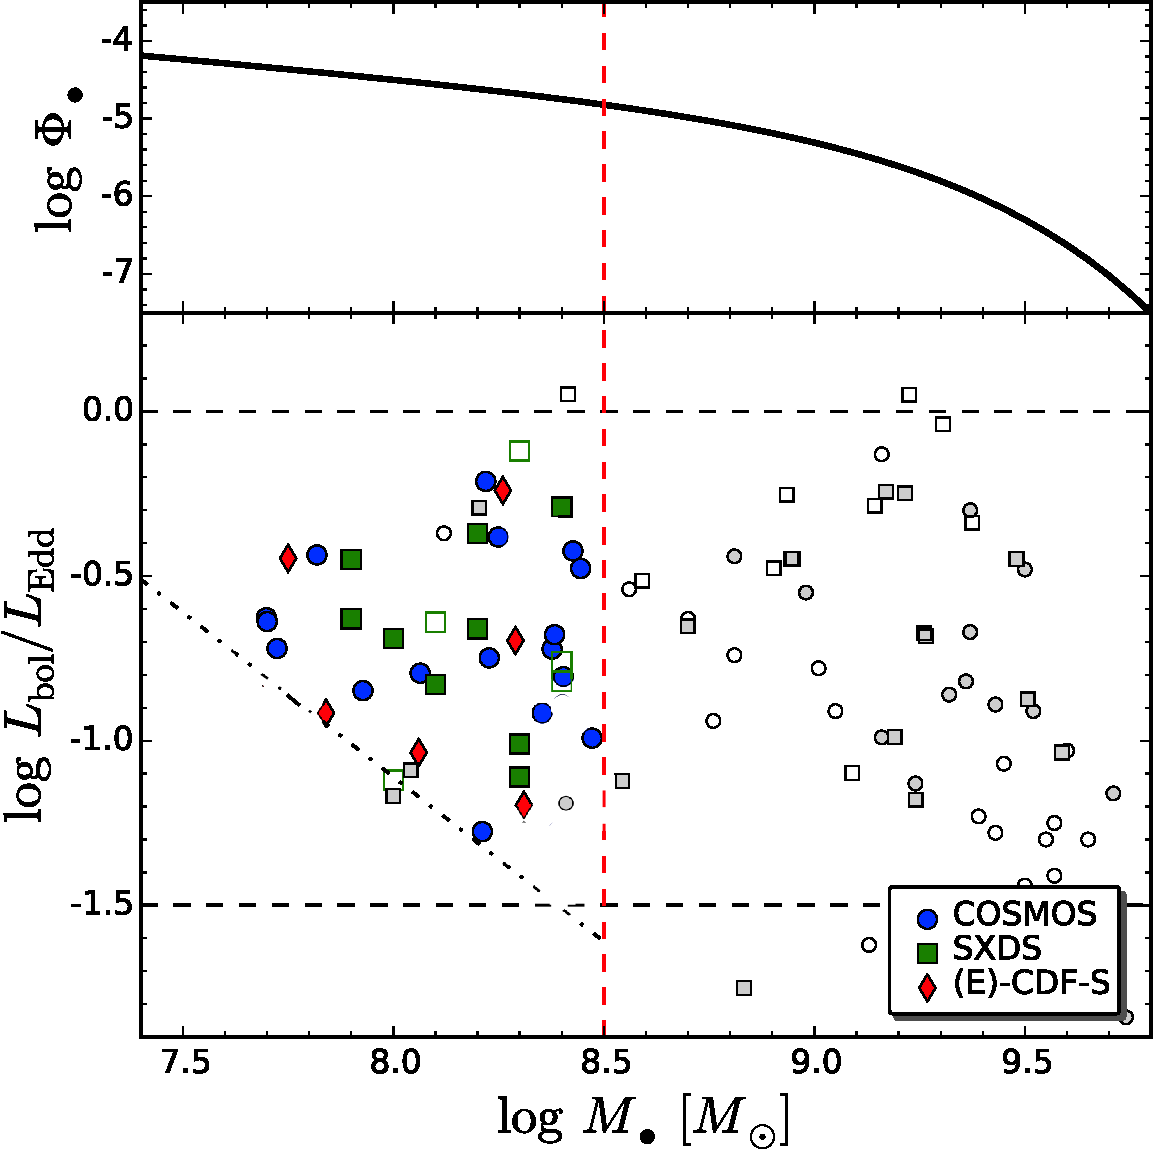
\includegraphics[width=0.8\linewidth]{hst_sample_bhmf.pdf}
%\caption{
%The selection function of our observation data. Eddington ratios (LBol/LEdd) and BH masses (bottom panel) of our sample (in color) that fall well-below the knee of the BH mass function at z = 1.5 (top panel; Schulze et al. 2015). Dashed lines (vertical and horizontal) denote our selection window with the slanted line only shown to approximately illustrate the effect of a luminosity limit, inherent in the parent catalogs. For reference, we indicate the high-z luminous SDSS QSO samples (grey squares - Peng et al. 2006; grey circles - Decarli et al. 2010) with all falling above our chosen upper mass limit.
%}
%\label{fig:support}
%\end{center}
%\end{figure}

\end{document}
